\documentclass[%
reprint,
%superscriptaddress,
%groupedaddress,
%unsortedaddress,
%runinaddress,
%frontmatterverbose, 
%preprint,
%preprintnumbers,
%nofootinbib,
%nobibnotes,
%bibnotes,
 amsmath,amssymb,
 aps,
%pra,
%prb,
%rmp,
%prstab,
%prstper,
%floatfix,
]{revtex4-2}

\usepackage{subfiles}
\usepackage{graphicx}% Include figure files
\usepackage{dcolumn}% Align table columns on decimal point
\usepackage{bm}% bold math
\usepackage{float}
\usepackage{mathtools}
\usepackage{xcolor}
%\usepackage{hyperref}% add hypertext capabilities
%\usepackage[mathlines]{lineno}% Enable numbering of text and display math
%\linenumbers\relax % Commence numbering lines

%\usepackage[showframe,%Uncomment any one of the following lines to test 
%%scale=0.7, marginratio={1:1, 2:3}, ignoreall,% default settings
%%text={7in,10in},centering,
%%margin=1.5in,
%%total={6.5in,8.75in}, top=1.2in, left=0.9in, includefoot,
%%height=10in,a5paper,hmargin={3cm,0.8in},
%]{geometry}

\newcommand{\Hp}{\mathcal{H}}
\renewcommand{\thesection}{\arabic{section}}
\renewcommand{\thesubsection}{\arabic{subsection}}
\renewcommand{\thesubsubsection}{\arabic{subsubsection}}

\begin{document}

\section{Milestone II}
Next we look at the recombination history of the universe. This is when baryons, mainly protons and electrons, went from being ionized to forming neutral atoms once the energy of the photons dropped below $13.6\,$eV. As a result, photons during this time decoupled from the thermal equilibrium of the universe and are what we now detect as the CMB photons. As this event is tightly related to the free mean path of photons, the goal of this section is to compute the optical depth $\tau$, the visibility function $\tilde g$ and their derivatives. In this project we only consider the formation of hydrogen and neglect the existence of any heavier atoms.

To accomplish this we start by calculating the free electron fraction $X_e$ which we will first compute from the Saha equation in early times till $X_e<0.99$ and then switch over to Peebles' equation from thereon. The reason we don't use Peebles' equation from the start is due to it being extremely sensitive to high temperatures and thus the solution at early times is very unstable.

\subsection{Theory}
As eluded to in the intro we will consider the optical depth $\tau(x)$ which is defined by the relation:
\begin{equation}
	I(r)=I_0e^{-\tau(r)},\label{eq:intensity}
\end{equation}
where $I_0$ is the intensity of a source which emits radiation and $I(r)$ is the intensity that an observer at a distance $r$ would detect. Here we can clearly see that if $\tau=0$ then $I(r)=I_0$ and thus the medium the radiation travels through does not affect the intensity. If $\tau\gg1$ then we say that the medium is optically thick and $\tau\sim1$ is the transition between the two.

In cosmology the main effect contributing to the optical depth is Thompson scattering of photons with free electrons. A more convenient form for the optical depth in the context of this text is:
\begin{equation}
	\tau(\eta)=\int_\eta^{\eta_0}d\eta'\,n_e\sigma_Ta,\label{eq:taueta}
\end{equation}
where $n_e$ is the number density of free electrons and $\sigma_T=\frac{8\pi}{3}\frac{\alpha^2\hbar^2}{m_e^2c^2}$ is the Thompson cross section which is found from QFT calculations. (\ref{eq:taueta}) can be rewritten into differential form:
\begin{equation}
	\frac{d\tau}{dx}=-\frac{cn_e\sigma_T}{H}, \label{eq:dtaudx}
\end{equation}
which is the ODE that we will solve. Since we see that the optical depth today is $0$ we have the initial condition $\tau(0)=0$. On the RHS of (\ref{eq:dtaudx}) the only missing factor is $n_e$. Instead of computing $n_e$ directly we will consider the fractional electron density:
\[X_e\equiv n_e/n_H\approx\frac{n_em_H}{\rho_b}=\frac{n_em_Ha^3}{\Omega_{\text{B}0}\rho_{c0}},\]
where the approximation is due to us not considering any heavier elements than hydrogen. To do this we consider the Saha equation:
\[\frac{n_en_p}{n_e^{(0)}n_p^{(0)}}=\frac{n_Hn_\gamma}{n_H^{(0)}n_\gamma^{(0)}},\]
Here $n_p,n_\gamma$ and $n_H$ are the number densities for free protons, photons and Hydrogen atoms respectively and $(0)$ represents that the given number density is in the thermal equilibrium. This is an analytical approximation for when the interaction rate is very high compared to the change in electron density. Since in the early universe consists purely of free electrons due to the high temperatures of the primordial plasma, this then suggests that the Saha equation is only valid when $X_e\approx 1$. Given our definition of $X_e$ and the approximations we can rewrite the Saha equation to the convenient form:
\begin{equation}
	\frac{X_e^2}{1-X_e}=\frac{1}{n_b}\left(\frac{k_bm_eT_b}{2\pi\hbar^2}\right)^{3/2}e^{-\epsilon_0/k_bT_b},
\end{equation}
where $T_b$ is the baryon temperature of the universe and $\epsilon_0=13.6\,\text{eV}$ is the ionization energy of hydrogen. In reality there should also be a $T_\gamma$ in this equation representing the temperature of photons at a given time, but in practice it is an excellent approximation to set $T_\gamma=T_b=T_{\text{CMB}0}/a$. The rewritten Saha equation is now simply a 2nd order polynomial in $X_e$ which is easily solved analytically:
\begin{align}
	X_e&=\frac{C}{2}\left[\sqrt{1+\frac{4}{C}}-1 \right],\label{eq:Saha}\\ 
	C&\equiv\frac{1}{n_b}\left(\frac{k_bm_eT_b}{2\pi\hbar^2}\right)^{3/2}e^{-\epsilon_0/k_bT_b},\label{eq:C}
\end{align}
where we have omitted the negative solution due to the electron fraction being manifestly positive. We also note that in the limit $4/C\ll1$ then $X_e=1$ which will be used in the numerical part later.

Since the Saha equation is only valid for $X_e\approx1$ then, as noted earlier, we consider Peebles' equation outside this realm. The derivation for Peebles' equation is beyond the scope of this paper and can be found at (cite x) and is given by:
\begin{equation}
	\frac{dX_e}{dx}=\frac{C_r(T_b)}{H}\left[\beta(T_b)(1-X_e)-n_HX_e^2\alpha^{(2)}(T_b)\right],\label{eq:Peebles}
\end{equation}
where
\begin{align*}
	C_r(T_b)&= \frac{\Lambda_{2s\rightarrow1s} +\Lambda_{\alpha}}{\Lambda_{2s\rightarrow1s} + \Lambda_{\alpha} +\beta^{(2)}(T_b)}, \\
	\Lambda_{2s\rightarrow1s}&= 8.227\,\text{s}^{-1},\\
	\Lambda_{\alpha}&= H\frac{(3\epsilon_0)^3}{(8\pi)^2 c^3\hbar^3 n_{1s}}, \\
	n_{1s}&= (1-X_e)n_H,\\
	n_H &= n_b, \,\,\text{(no helium)}\,\,\,\color{red}(*)\color{black}\\
	n_b &= \frac{3H_0^2 \Omega_{b0}}{8\pi G m_H a^3},\\
	\beta^{(2)}(T_b) &= \beta(T_b) e^{\frac{3\epsilon_0}{4k_bT_b}},\\
	\beta(T_b) &= \alpha^{(2)}(T_b) \left(\frac{m_ek_bT_b}{2\pi \hbar^2}\right)^{3/2} e^{-\frac{\epsilon_0}{k_bT_b}},\\
	\alpha^{(2)}(T_b)&= \frac{8}{\sqrt{3\pi}}	c\sigma_T\sqrt{\frac{\epsilon_0}{k_bT_b}}\phi_2(T_b),\\
	\phi_2(T_b)&= 0.448\ln\left(\frac{\epsilon_0}{k_bT_b}\right).
\end{align*}
\color{red}$(*)$ Shouldn't $n_H=n_b/2$ if we include electrons into our definition of baryons with the assumptions that there are equally many protons as electrons? Or are we suddenly switching over to the particle physics definition of baryons? \color{black}This ODE will then be solved numerically to find $X_e(x)$ with the initial condition given from the last $X_e$ value from the Saha solution. This then gives us $n_e(x)$ from the definition of $X_e$ which will then be used to solve (\ref{eq:dtaudx}) for $\tau(x)$.

Further we consider the visibility function:
\begin{equation}
	\tilde g(x)\equiv\frac{d}{dx}e^{-\tau(x)}=-e^{-\tau(x)}\tau'(x), \label{gtilde}
\end{equation}
which describes the probability density for a given photon to having its final scattering at time $x$. Since this is a probability density then it must satisfy
\[\int_{-\infty}^0dx\,\tilde g(x)=1\]
The visibility function can be thought of as the probability that a photon scattering between time $x$ and $x+dx$ is the last time it ever scatters before it moves freely. From this we can then consider \textbf{last scattering} to occur when the visibility function peaks. The solution to $\tau(x)$ and its derivative makes getting the visibility function a trivial task.

Finally we have the sound-horizon $s(x)$ which is given by:
\begin{align}
	s(x)\equiv\int_0^adt\,\frac{c_s}{a}, \label{soundhor}
\end{align}
where $c_s=c\sqrt{\frac{R}{3(1+R)}}$ is the sound-speed of the coupled photon-baryon plasma and $R=\frac{4\Omega_{\gamma0}}{3a\Omega_{\text{B}0}}$. We can rewrite (\ref{soundhor}) into a differential form as such:
\begin{equation}
	\frac{ds}{dx}=\frac{c_s}{\Hp},
\end{equation}
with the initial condition $s(x_{\text{ini}})=\frac{c_s(x_{\text{ini}})}{\Hp(x_{\text{ini}})}$. 



\subsection{Implementation details}
\subsubsection{Solving the Saha and Peebles' equation}
We began by implementing a for-loop for the Saha equation which at each iteration checks whether we are still in the Saha regime. Note that we have to be careful about round-off errors when solving the Saha equation when the term $\epsilon_0/k_bT_b$ in the exponential in (\ref{eq:C}) goes to very small values the rest of the expression will begin to explode. Thus in (\ref{eq:Saha}) we would be subtracting two very large numbers which should at the end simplify to just $1$ leading to potential round-off errors. To avoid this we instead performed an \texttt{if}-test to check whether $4/C$ is less than some small threshold. Once this is the case then we simply set $X_e$ to $1$. A justification for this can be seen by considering the first order expansion of the square root in (\ref{eq:Saha}), which will just yield $X_e=1$. Since the Saha equation is only valid for $X_e\approx1$ we decide to switch over to the more accurate Peebles' equation $X_e<0.99$. For reference we continued on with the Saha equation past its validity to compare the results. 

Peebles' equation was then solved numerically via the same ODE solver used in the previous milestone with the initial condition supplied by the last point before we exited the Saha regime. Some care was taken to ensure no overflow due to the exponential in the $\beta^{(2)}$ equation under (\ref{eq:Peebles}). To do this we simply created another \texttt{if}-test to check when the term in the exponential exceeded 150 and set $\beta^{(2)}=0$ as the exponential from $\beta$ will dominate over it. We then had the results for $X_e$ which we used to compute $n_e$ for both cases. The results for both the Saha only and the Saha-Peebles computations were splined and printed to a data file.
\subsubsection{Solving for the optical depth and visibility functions}
Next we solved the ODE for both the optical depth $\tau(x)$ in eq. \ref{eq:dtaudx} and the sound-horizon $s(x)$ with the before mentioned initial conditions. Note that the prior ODE, if computed it in the usual way, one would need to subtract an initial condition off the solution for $\tau(x=0)$ which would lead to round-off errors close to $x=0$ due to the finite precision of floating point numbers. This would then lead to noise in the solution and thus the ODE was then instead solved by going backwards in time to avoid this problem. After, $\tau'(x)$ was also computed since the spliner we are working with seemingly does not work well past 1st derivatives since we also want to look at $\tau''(x)$. With both $\tau(x)$ and $\tau'(x)$ we could easily calculate the visibility function $\tilde g(x)$ with (\ref{gtilde}) and its first derivative. These were then all splined along with using the \texttt{deriv\_x} function in the spliner s.t. we have access to the 2nd derivatives. All the data was again printed to the aforementioned data file.

With the various splines we then calculated the time at recombination and last scattering. Our definition for when recombination happens is when $X_e$ drops below 0.1. We have 2 different definitions for when last scattering occurred; when $\tilde g$ peaks and when $\tau=1$. This was done by iterating through the data in \texttt{C++} until these conditions were met.

\subsubsection{Python}
As before the data was imported to Python and various plots together with a table of the various events were made.

\subsection{Results}
\subsubsection{Recombination Events}
We first consider the quantities $x,z,y$ and $r_s$ at both recombination and when last scattering occurred. The results are summarized in TABLE \ref{tab:recombination_events} where ``w/ $\tau$'' refers to the definition of last scattering where $\tau=1$. This seems to give the result that last scattering happened before recombination. This is of course unreasonable as recombination causes last scattering to occur, thus for future reference the peak of $\tilde g$ will be chosen as our definition for last scattering. \color{red}[I don't entirely see the point in even considering $\tau=1$ as the definition as its quite arbitrary. I sort of want to create some argument for why to exclude it as it does not make much sense regarding the theory. In the end I find that I really just want to exclude any mention of it entirely but since it was mentioned in the milestone text I figured that we are expected to comment on it.]  \color{black}The times for recombination and last scattering both are in agreement previously found values (cite x,y,z).
\renewcommand{\arraystretch}{1.25}
\begin{table}[ht!]
	\caption{Recombination Events}
	\label{tab:recombination_events}
	\begin{tabular}{|l|c|c|c|c|}
		\hline
		Event                               & $x$       & $z$      & $t$ [kyr] & $r_s$ [Mpc] \\\hline
		Recombination                & $-6.9855$ & $1079.8$ & $377.96$  & $145.278$   \\\hline
		Last scattering                 & $-6.9853$ & $1079.7$ & $378.04$  & $145.292$   \\\hline
		Last scattering w/ $\tau$ & $-6.9878$ & $1082.3$ & $376.51$  & $145.062$   \\\hline
	\end{tabular}
\end{table}
\subsubsection{Electron Fraction $X_e$}
The results for the electron fraction $X_e$ are given in FIG. \ref{fig:Xe}. Here we see that the moment the electron fraction deviates even a small amount from $X_e=1$ then the Saha equation plummets, suggesting that recombination would happen at some time $x\sim-7.14$ instead of the value given in TABLE \ref{tab:recombination_events} with Peebles' more accurate equation. In this figure, freeze out refers to the present day abundance of free electron which we find to be $X_e(0)\approx2.03\cdot10^{-4}$. 
\begin{figure}[ht!]
\caption{Time evolution of the free electron fraction $X_e(x)$.}
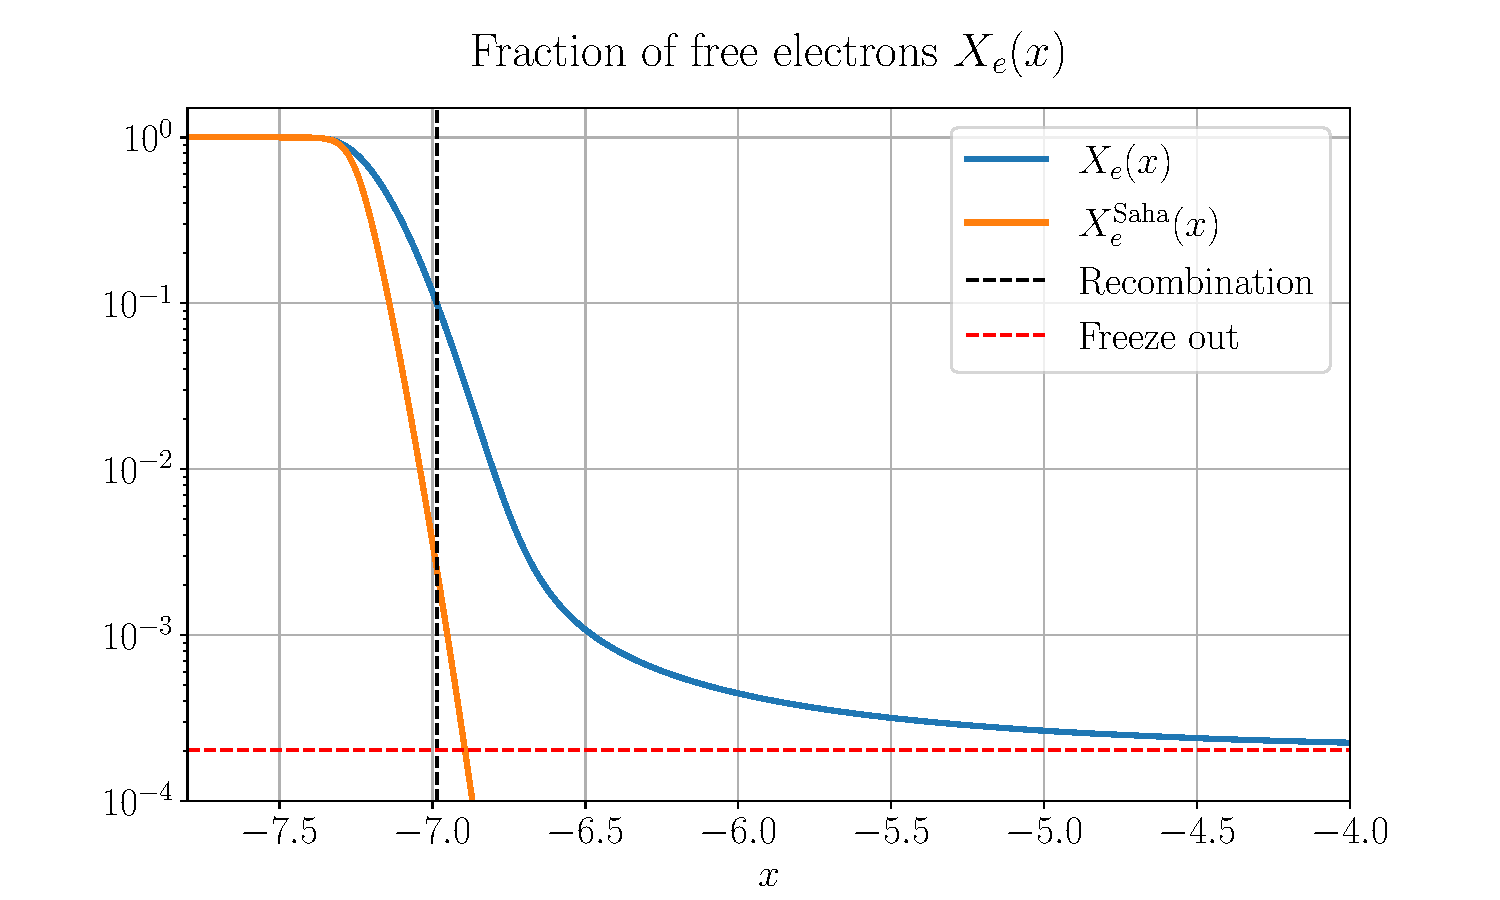
\includegraphics[width = \linewidth]{Figures/Xe.pdf}
\label{fig:Xe}
\end{figure}
\subsubsection{Evolution of Optical Depth and Visibility function}
Further we consider the time evolution of the optical depth parameter, the visibility function and their derivatives given in FIG. \ref{fig:tau} and \ref{fig:gtilde} respectively. The negative of the first derivative of $\tau$ is plotted s.t. we can read off all of them in a single log-plot and for a similar reason the derivatives of $\tilde g$ are normalized such that their peak is at $\max\tilde g$. The surface of last scattering with the $\tilde g$ peak definition is shown for reference. 

\begin{figure}[ht!]
	\caption{Time evolution of the optical depth $\tau(x)$ and its derivatives.}
	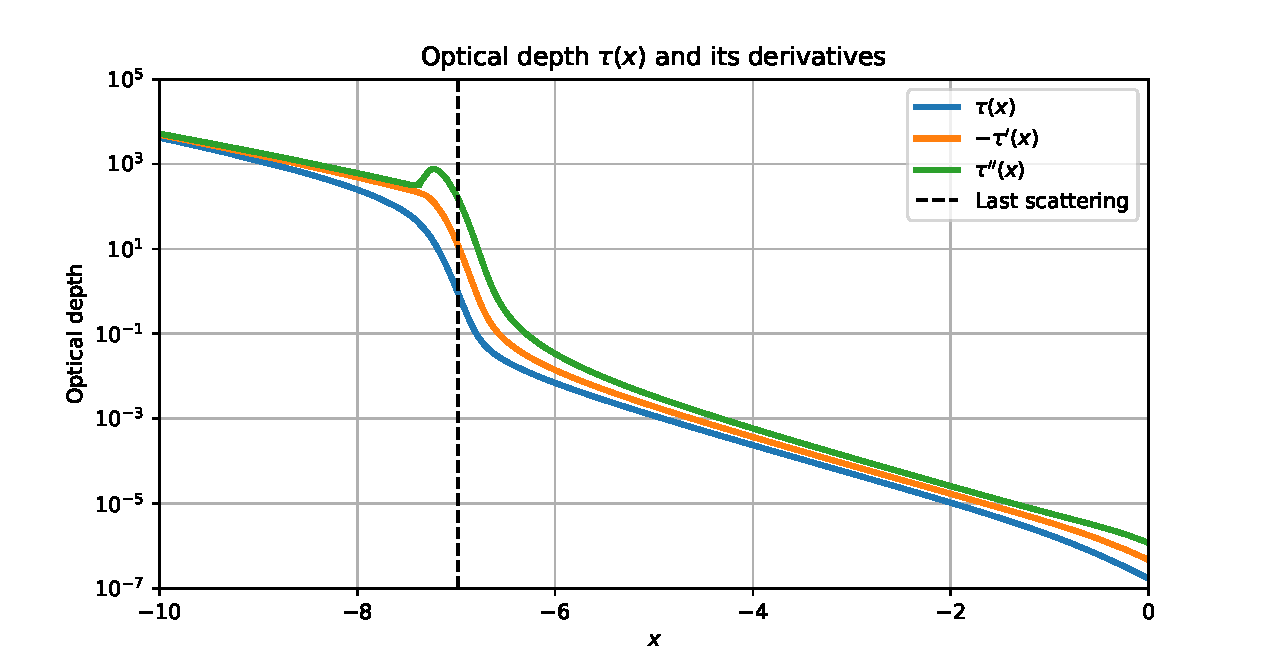
\includegraphics[width = \linewidth]{Figures/tau_and_derivs.pdf}
	\label{fig:tau}
\end{figure}
\begin{figure}[ht!]
	\caption{Time evolution of visibility function $\tilde g$ and its derivatives all normalized s.t. $\max|\tilde g|=\max|\tilde g'|=\max|\tilde g''|$ So that it all fits in the same plot. These scale factors are roughly $10$ and $200$ for $\tilde g'$ and $\tilde g''$ respectively.}
	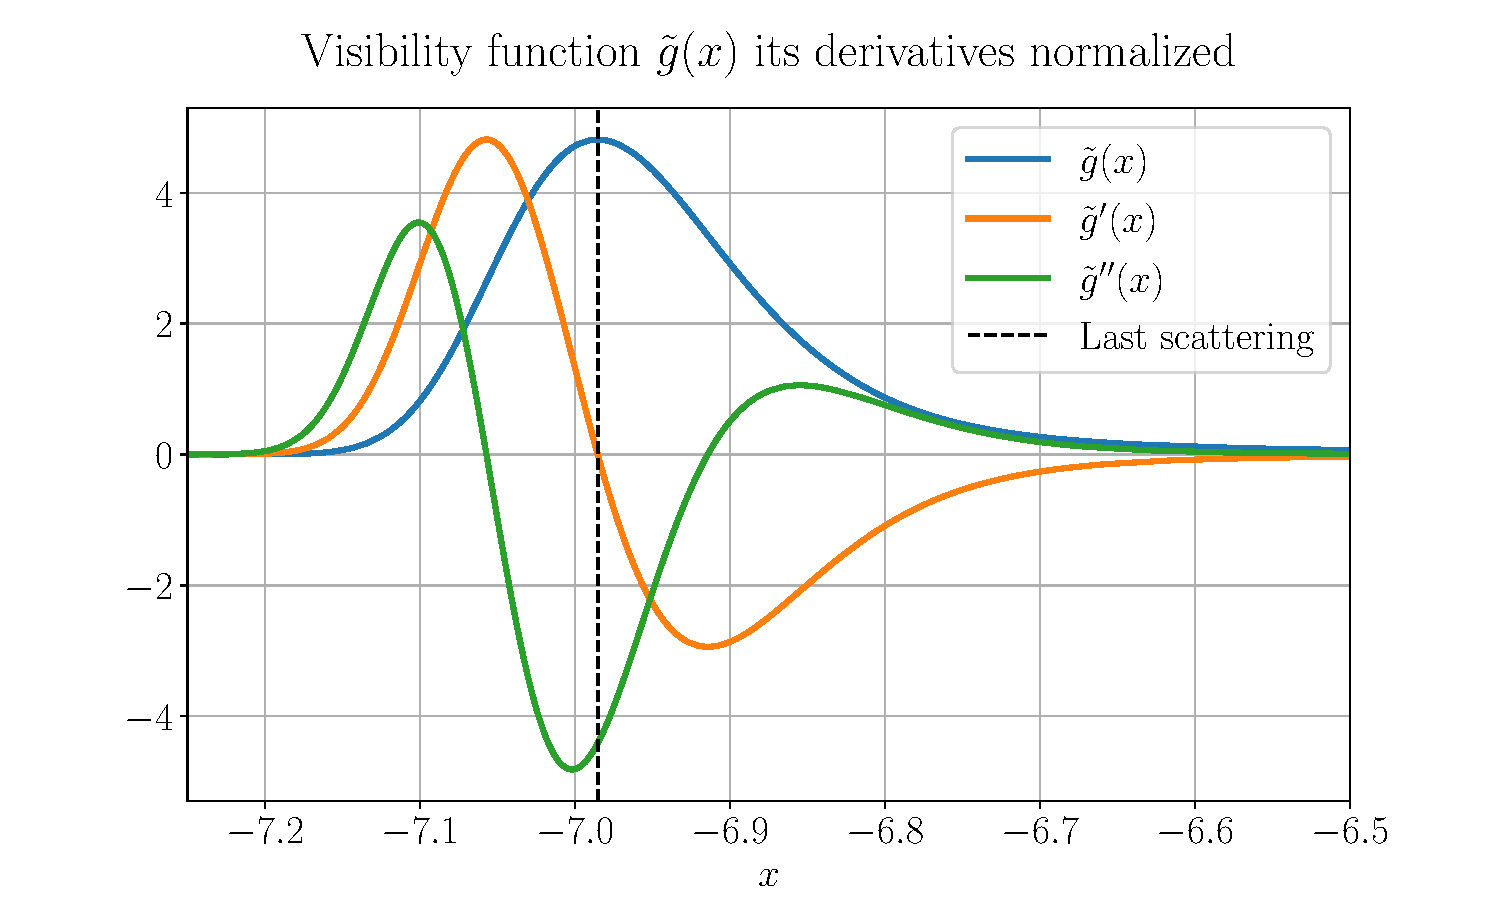
\includegraphics[width = \linewidth]{Figures/gtilde.pdf}
	\label{fig:gtilde}
\end{figure}

Before this dashed line signaling the last scattering event, the primordial plasma is optically thick, thus the mean free path of photons is too short and will continue on scattering. However, the optical depth at this time still endures a stable decay almost solely due to the expansion rate of the universe as this causes the number density $n_e$ to decrease. This relation can be seen in (\ref{eq:taueta}). As mentioned previously, the visibility function is the probability density that a given photon had its last scattering at time $x$. Thus we can see that when the optical depth is very high, the likelihood of a particular photon at that time scattering for the last time is very small. 

$\tau(x)$ then dips down violently as the number of free electrons in the universe rapidly decays. At the same time we then see that this is when the visibility function begins to rapidly increase. This  clearly shows that the formation of neutral Hydrogen happens much faster than the expansion of the universe, hence having the largest effect in this epoch. This in turn means that the mean free paths of photons increase beyond the horizon and thus, photons are effectively free to travel without interacting with matter. This is then the last scattering event and the photons released here are the ones that we detect today in the CMB spectra. 

Once the electron fraction begins to flatten out again, the optical depth becomes a straight line on the log-plot, once again caused by the expansion of the universe. The visibility function also begins to flatten out at this point, albeit at a slower rate than the initial increase before last scattering. 


\subsection{Conclusion}
We can readily note from FIG. \ref{fig:gtilde} that recombination and last scattering did not happen instantaneously, as $\tilde g(x)$ would take the form of a Dirac-delta function, but instead over a relatively short period of time. Due to the short time frame, the number of free electrons in the universe rapidly decreased over several orders of magnitude. The values in TABLE \ref{tab:recombination_events} show us that recombination generally happens first, with the last scattering following shortly after.

As expected from the assumptions made in the derivation of the Saha equation, we see that it quickly becomes a terrible approximation outside of its regime. The manifestly seen correlation between the change in fraction of free electrons, optical depth and the visibility function is also clearly seen, but is of no surprise from their various relations.


\end{document}